\section{\xxx Overview} \label{sec:overview}

Figure 2 shows \xxx's architecture. The replication logic is entirely 
implemented in qemu-kvm, a KVM tailored version of QEMU. It contains 
two main components: 
The protocol interposes on \tapsend on receiving a network packet and runs 
a consensus process on this request. Besides, this component maintains a 
packet queue to capture outgoing packets by interposing on \taprecv and invokes 
the output checking protocol periodically.

% On receiving a packet, QEMU calls tap_send()
% On sending a packet, QEMU calls tap_receive()
% We maintain a packet queue to capture outgoing packets.

\begin{figure}[t]
% \vspace{.20in}
\centering
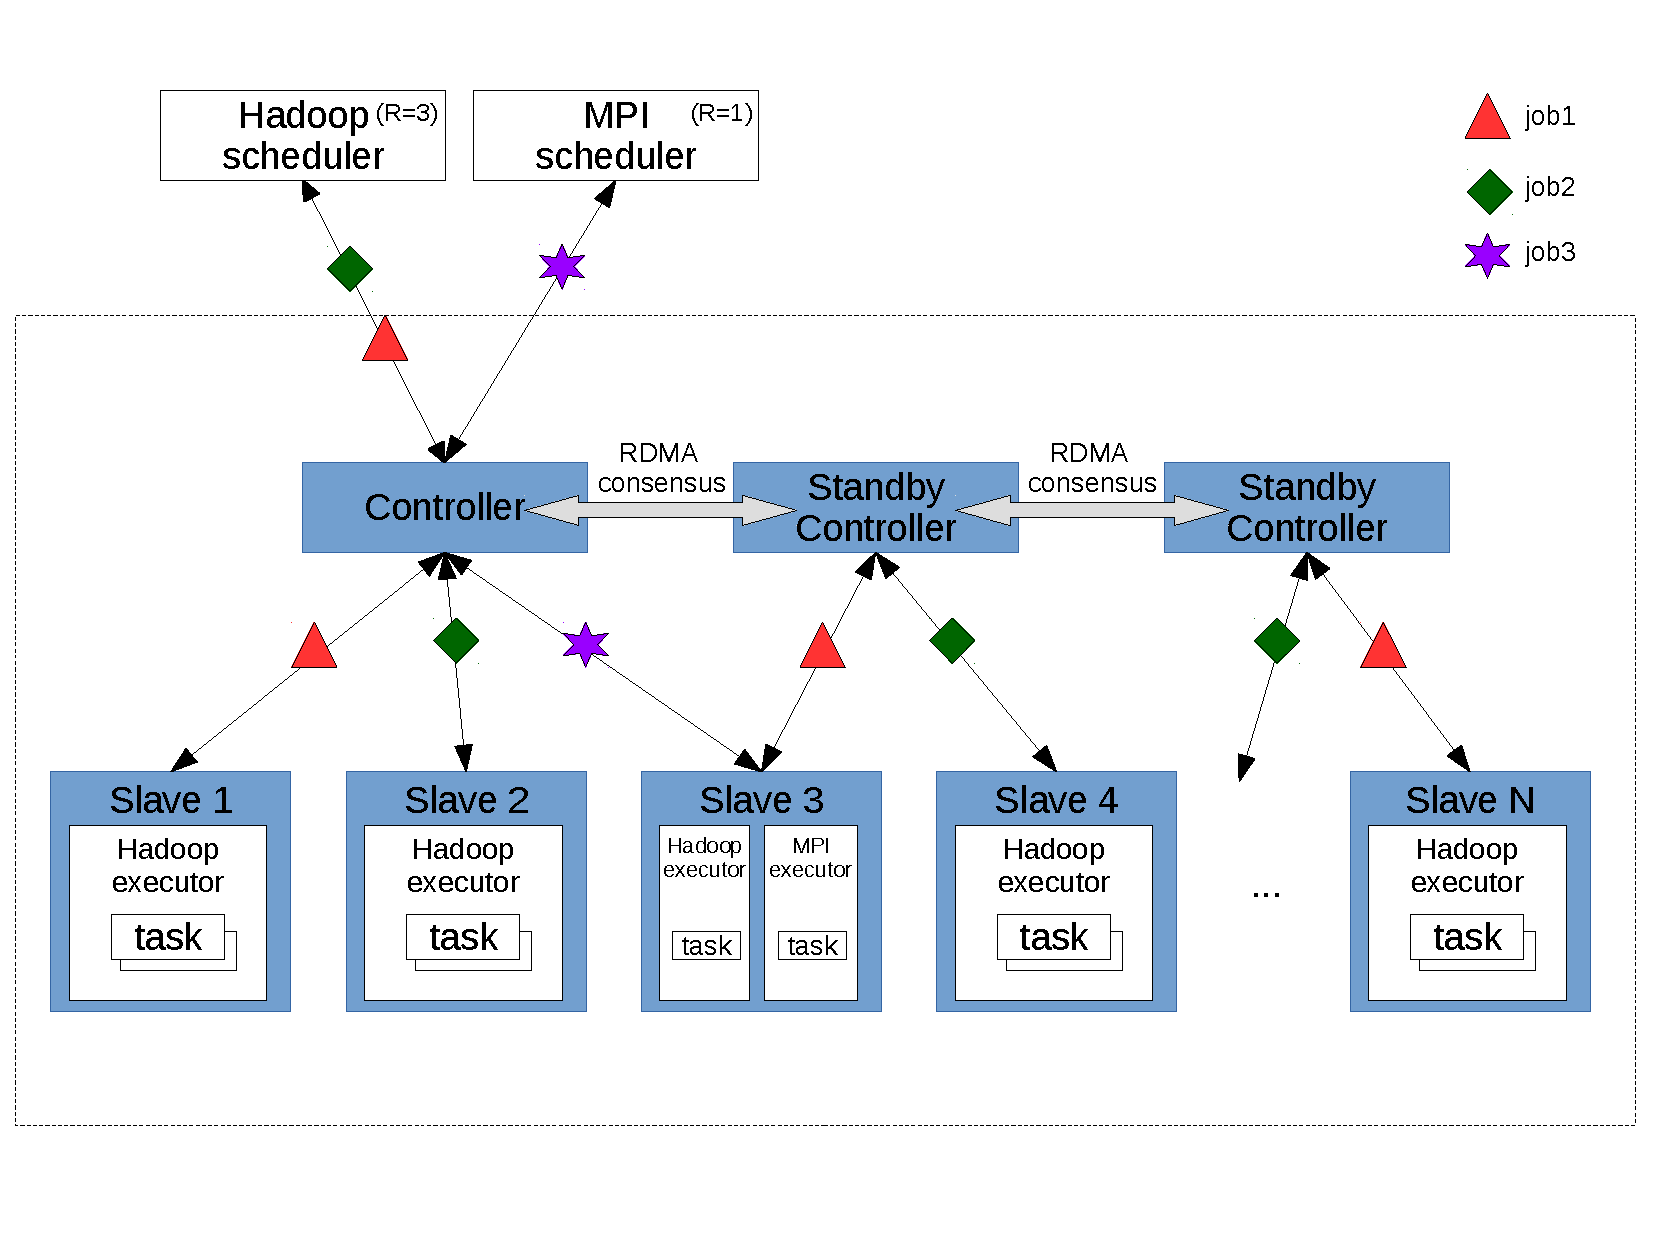
\includegraphics[width=.47\textwidth]{figures/arch}
\vspace{-.2in}
\caption{{\em The \xxx Architecture.}} \label{fig:arc}
\vspace{.05in}
\end{figure}
